\documentclass{article}
\usepackage[utf8]{inputenc}
\usepackage{tikz}
\usetikzlibrary{positioning}
\usetikzlibrary{shapes}

\begin{document}

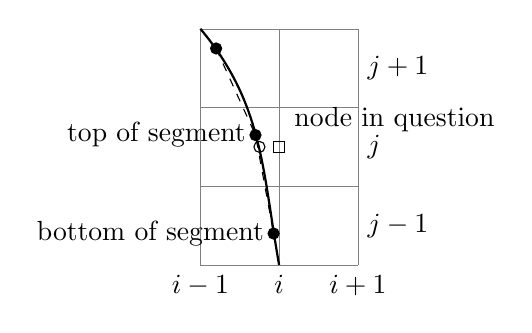
\begin{tikzpicture}

%grid
\draw[step=1cm,gray,very thin] (-1,-1) grid (1,2);
%body
\draw[black, thick]    (0,-1) to[out=100,in=-50] (-1,2);
%Lagrangian body
\filldraw [black] (-0.8,1.75) circle (2pt);
\filldraw [black] (-0.3,0.65) circle (2pt) node[anchor=east]{top of segment};
\filldraw [black] (-0.07,-.6) circle (2pt) node[anchor=east]{bottom of segment};
%line between segments
\draw [black, thin, dashed] (-0.8,1.75) -- (-0.3,0.65) -- (-0.07,-0.6);
%HN
\draw [black] ([xshift=-2pt,yshift=-2pt]0,0.5) rectangle ++(4pt,4pt) node[anchor=south west]{node in question};
%BI
\draw [black] (-0.25,0.5) circle (2pt) node[anchor=east] {};
%i,j indicators
\node[anchor=north] at (-1,-1) {$i-1$};
\node[anchor=north] at (0,-1) {$i$};
\node[anchor=north] at (1,-1) {$i+1$};
\node[anchor=west] at (1,1.5) {$j+1$};
\node[anchor=west] at (1,0.5) {$j$};
\node[anchor=west] at (1,-0.5) {$j-1$};

\end{tikzpicture}


\end{document}
